\chapter{Технологическая часть}

\section{Средства реализации программы}

В качестве языка программирования для реализации курсовой работы был выбран язык C++~\cite{C++} по следующим причинам:

\begin{itemize}
	\item В стандартной библиотеке языка присутствует поддержка всех
	структур данных, выбранных по результатам проектирования;
	\item высокая производительность;
	\item наличие фреймворка Qt~\cite{Qt}
	\item большое количество актуальной документации.
\end{itemize}

\section{Реализация алгоритмов}

На листингах~\ref{lst:terr},~\ref{lst:ds} представлен код ключевых классов программного обеспечения.

\begin{lstlisting}[label=lst:terr,caption=Класс ландшафта]
class Terrain
{
	private:
	Matrix<double> height_mtr;
	Matrix<QVector3D> screen_mtr;
	
	vector<QVector3D> normal_plains;
	vector<double> intensity;
	
	double max_height;
	double min_height;
	
	double water_level = 0;
	
	QVector3D center_;
	
	QVector3D corrector_vector = {0, 0, 1};
	
	
	public:
	explicit Terrain(): Terrain(0)
	{
	}
	
	explicit Terrain(size_t n): max_height(INT_MIN), min_height(INT_MAX)
	{
		height_mtr.resize(n);
		for (auto &v: height_mtr)
		v.resize(n);
		
		screen_mtr.resize(n);
		for (auto &v: screen_mtr)
		v.resize(n);
	}
	
	Matrix<QVector3D> &get_screen_matrix()
	{
		return screen_mtr;
	}
	
	const Matrix<QVector3D> &get_screen_matrix() const
	{
		return screen_mtr;
	}
	
	const Matrix<double> &get_height_matrix() const
	{
		return height_mtr;
	}
	
	Matrix<double> &get_height_matrix()
	{
		return height_mtr;
	}
	
	vector<QVector3D> &get_normal_matrix()
	{
		return normal_plains;
	}
	
	vector<double> &get_intensity_matrix()
	{
		return intensity;
	}
	
	const vector<double> &get_intensity_matrix() const
	{
		return intensity;
	}
	
	const vector<double> &operator[](size_t index) const
	{
		return height_mtr[index];
	}
	
	vector<double> &operator[](size_t index)
	{
		return height_mtr[index];
	}
	
	size_t size() const
	{
		return height_mtr.size();
	}
	
	double get_max_h() const
	{
		return max_height;
	}
	
	void set_max_h(double h)
	{
		max_height = h;
	}
	
	double get_min_h() const
	{
		return min_height;
	}
	
	void set_min_h(double h)
	{
		min_height = h;
	}
	
	void set_center(const QVector3D& vector_)
	{
		center_ = vector_;
	}
	
	QVector3D& get_center()
	{
		return center_;
	}
	
	void clear();
	
	void intensity_clear()
	{
		intensity.clear();
		intensity.resize(0);
	}
	
	QVector3D& get_v_corrector()
	{
		return corrector_vector;
	}
	
	double get_water_level() const
	{
		return water_level;
	}
	
	void set_water_level(double water_level)
	{
		this->water_level = water_level;
	}
	
};
\end{lstlisting}

\clearpage

\begin{lstlisting}[label=lst:ds,caption=Реализация алгоритма diamond-square]
static random_device rd;
static mt19937 random_generator;

void Diamond_Square::init_rand_dev()
{
	random_generator.seed(rd());
}


double Diamond_Square::random(double noise)
{
	uniform_real_distribution<double> distribution{-noise, noise};
	return distribution(random_generator);
}


void Diamond_Square::diamond_step(Terrain &terrain, int step_wide, double noise)
{
	int neighbour_dist = step_wide / 2;
	vector<pair<int, int> > diamond_offset = {{-1, -1}, {-1, 1}, {1, 1}, {1, -1}};
	
	for (size_t row = neighbour_dist; row < terrain.size(); row += step_wide)
	{
		for (size_t col = neighbour_dist; col < terrain.size(); col += step_wide)
		{
			terrain[row][col] = strategy->avg(terrain, row, col, neighbour_dist, diamond_offset) + random(noise);
			terrain.set_max_h(max(terrain.get_max_h(), terrain[row][col]));
			terrain.set_min_h(min(terrain.get_min_h(), terrain[row][col]));
		}
	}
}

void Diamond_Square::diamond_step_row(Terrain &terrain, int step_wide, double noise)
{
	int neighbour_dist = step_wide / 2;
	vector<pair<int, int> > square_offset = {{-1, 0}, {0, -1}, {1, 0}, {0, 1}};
	
	for (size_t row = neighbour_dist; row < terrain.size(); row += step_wide)
	{
		for (size_t col = 0; col < terrain.size(); col += step_wide)
		{
			terrain[row][col] = strategy->avg(terrain, row, col, neighbour_dist, square_offset) + random(noise);
			terrain.set_max_h(max(terrain.get_max_h(), terrain[row][col]));
			terrain.set_min_h(min(terrain.get_min_h(), terrain[row][col]));
		}
	}
}

void Diamond_Square::diamond_step_col(Terrain &terrain, int step_wide, double noise)
{
	int neighbour_dist = step_wide / 2;
	vector<pair<int, int> > square_offset = {{-1, 0}, {0, -1}, {1, 0}, {0, 1}};
	
	for (size_t row = 0; row < terrain.size(); row += step_wide)
	{
		for (size_t col = neighbour_dist; col < terrain.size(); col += step_wide)
		{
			terrain[row][col] = strategy->avg(terrain, row, col, neighbour_dist, square_offset) + random(noise);
			terrain.set_max_h(max(terrain.get_max_h(), terrain[row][col]));
			terrain.set_min_h(min(terrain.get_min_h(), terrain[row][col]));
		}
	}
}

Terrain Diamond_Square::generate_terrain()
{
	Terrain terrain(n);
	
	int step_wide = n;
	double rand_noise = 1;
	
	while (step_wide > 1)
	{
		diamond_step(terrain, step_wide, rand_noise);
		diamond_step_row(terrain, step_wide, rand_noise);
		diamond_step_col(terrain, step_wide, rand_noise);
		
		step_wide /= 2;
		rand_noise *= smooth;
	}
	
	return terrain;
}
\end{lstlisting}

\clearpage

\section{Интерфейс программы}

Интерфейс программы представлен на рисунке~\ref{fig:interface}.

\begin{figure}[H]
	\centering
	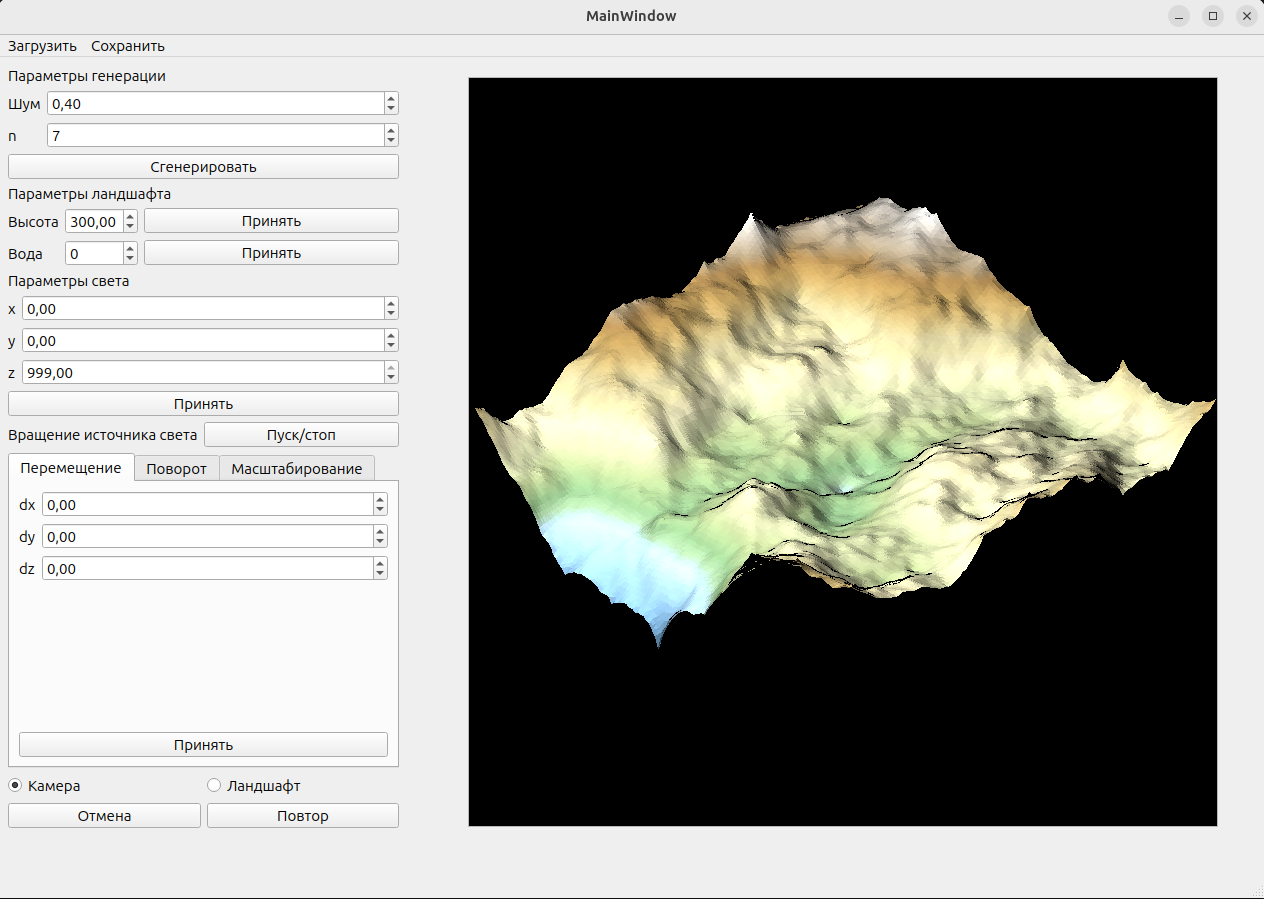
\includegraphics[height=0.45\textheight]{interface.png}
	\caption{Интерфейс программного обеспечения}
	\label{fig:interface}
\end{figure}

\section*{Вывод}

В данном разделе были выбраны средства реализации для программного обеспечения, и предоставлены реализации разработанных алгоритмов. Также описан графический интерфейс.